\documentclass[11pt,a4paper]{article}

\usepackage[margin=2.0cm]{geometry}
\usepackage{amsmath,amssymb,amsfonts}
\usepackage[T1]{fontenc}
\usepackage{lmodern}
\usepackage{microtype}
\usepackage{enumitem}
\usepackage{booktabs}
\usepackage{tabularx}
\usepackage{xcolor}
\usepackage[hidelinks,colorlinks=true,
            urlcolor=blue!50!black,linkcolor=blue!50!black]{hyperref}
\usepackage{listings}
\usepackage{tikz}
\usepackage{pgfplots}
\pgfplotsset{compat=1.18}
\usetikzlibrary{positioning,arrows.meta,shapes.geometric,fit,calc,
                decorations.pathreplacing,backgrounds}

\definecolor{matclr}{RGB}{40,103,160}
\definecolor{unitclr}{RGB}{180,70,40}
\definecolor{rawclr}{RGB}{50,140,80}
\definecolor{prodclr}{RGB}{160,60,140}
\definecolor{kept}{RGB}{40,140,80}
\definecolor{cut}{RGB}{170,60,60}
\definecolor{accent}{RGB}{200,120,30}
\definecolor{regimeA}{RGB}{120,170,210}
\definecolor{regimeB}{RGB}{60,130,170}
\definecolor{regimeC}{RGB}{200,120,30}
\definecolor{regimeD}{RGB}{170,60,40}

\tikzset{
  mat/.style={circle,draw=matclr,thick,fill=matclr!10,
              minimum size=8mm,inner sep=0.5pt,font=\scriptsize},
  raw/.style={mat,draw=rawclr,fill=rawclr!12},
  prod/.style={mat,draw=prodclr,fill=prodclr!12,line width=0.5mm},
  unit/.style={rectangle,draw=unitclr,thick,fill=unitclr!10,
                minimum height=7mm,minimum width=18mm,
                rounded corners=1pt,inner sep=1pt,font=\scriptsize},
  unitin/.style={unit,fill=kept!22,draw=kept!80},
  edge/.style={-{Stealth[length=1.6mm]},semithick},
}

\lstset{
  basicstyle=\ttfamily\footnotesize,
  breaklines=true, columns=fullflexible, keepspaces=true,
  showstringspaces=false, frame=single, rulecolor=\color{gray!30},
}

\newcommand{\HyMeKo}{\textsc{HyMeKo}}
\newcommand{\code}[1]{\texttt{\small #1}}
\setlist[itemize]{leftmargin=1.4em,itemsep=2pt,topsep=3pt}
\setlist[enumerate]{leftmargin=1.6em,itemsep=2pt,topsep=3pt}

\title{P-graph ABB for neural-architecture search\\[3pt]
       \large\normalfont
       seven Pareto-optimal HSiKAN configurations from one DSL
       and one $\boldsymbol{w}$-sweep}
\author{Companion to the Pimentel multi-objective dossier}
\date{2026-05-19}

\begin{document}
\maketitle

\begin{center}
\fbox{\begin{minipage}{0.93\linewidth}\small
\textbf{In one sentence.} The same multi-objective $\mathrm{ABB}$
that selects a methanol-synthesis plant now selects a Pareto-optimal
HSiKAN signed-link-prediction architecture: 11 operating units
across cycle-enumeration, backbone-width, training-schedule, and
mandatory-evaluation choice axes; 4 cost dimensions
\textsf{(auc\_gap, gpu\_gb, params\_m, wall\_min)}; \textbf{seven
structurally distinct optimal configurations} across the weight
space, spanning a $7\times$ resource range for a ${\sim} 0.08$ AUC
range, with the AUC-paramount endpoint coinciding exactly with our
2026-05-13 Optuna-best 10-seed SOTA configuration.
\end{minipage}}
\end{center}

\vspace{4pt}

% ===================================================================
\section{The mapping: NN architecture as a P-graph}

\begin{center}\small
\begin{tabular}{p{0.36\linewidth} p{0.58\linewidth}}
\toprule
P-graph concept & NN-architecture-search analogue \\
\midrule
Materials $M$                & Resource budgets $+$ intermediate quality artefacts \\
Raw materials $R$            & GPU budget, wall-clock budget \\
Product demand $P$           & Validated trained model (passes 5-seed eval) \\
Operating units $O$          & Architecture choices: cycle-enum, backbone, training, eval \\
$\mathrm{in}(u), \mathrm{out}(u)$ & Resources $u$ consumes; quality it produces \\
Cost vector $\boldsymbol{c}(u)$  & per-unit \textsf{(auc\_gap, gpu\_gb, params\_m, wall\_min)} \\
Weight vector $\boldsymbol{w}$   & Project priority across the 4 dimensions \\
Inclusion bound              & Total weighted cost $\geq$ incumbent $\Rightarrow$ prune \\
Reachability bound           & Can optimistic remainder still produce a validated model? \\
\textbf{ABB optimum}         & \textbf{Pareto-optimal architecture for this $\boldsymbol{w}$} \\
\bottomrule
\end{tabular}
\end{center}

\paragraph{Why the framework applies.} Theorem~1 of the formalism
extension (admissibility under positive-weighted scalarisation)
requires the cost vector $\boldsymbol{c}(u) \in \mathbb{R}_{\geq 0}^D$.
\textsf{auc\_gap} is a non-negative cost (it measures the per-unit
contribution to the gap below the headline 0.9959 Optuna-best AUC,
treated as approximately additive); all three resource dimensions
are obviously non-negative. The reachability bound is structural
and survives intact.

\paragraph{Why this is not Optuna.}
\begin{center}\small
\begin{tabularx}{0.98\linewidth}{lXX}
\toprule
 & Optuna (gradient-free Bayesian) & P-graph multi-objective ABB \\
\midrule
Search & sampling over a continuous space & exhaustive over a discrete subset lattice \\
Multi-objective & scalarised loss only & native, weights at query time \\
Feasibility & implicit & explicit (reachability bound) \\
Pareto front & post-hoc inference & first-class (sweep $\boldsymbol{w}$) \\
Best for & exploring a vast space & curating a known catalogue \\
\bottomrule
\end{tabularx}
\end{center}
The two are complementary. ABB is the right tool when the
catalogue is curated (the case for established architectures like
HSiKAN-mixed-arity) and the user wants the structural justification
the inclusion/reachability bounds provide.

% ===================================================================
\section{The HSiKAN architecture P-graph}

\subsection{Topology}

\begin{center}
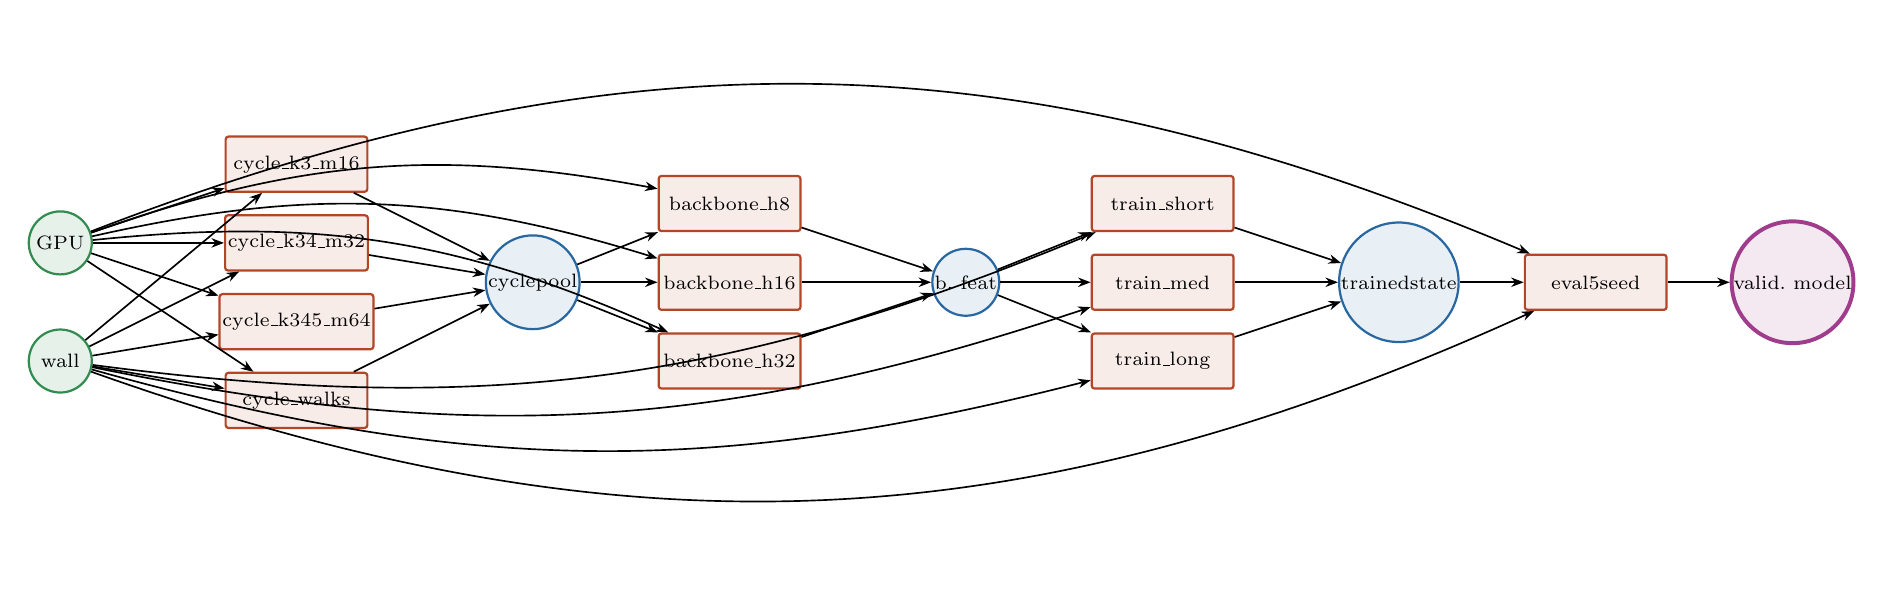
\begin{tikzpicture}[node distance=4mm and 12mm]
% Raws (left)
\node[raw] (gpu)  at (0,2.0) {GPU};
\node[raw] (wall) at (0,0.5) {wall};

% Cycle enum (4 alternatives)
\node[unit] (c1) at (3,3.0)  {cycle\_k3\_m16};
\node[unit] (c2) at (3,2.0)  {cycle\_k34\_m32};
\node[unit] (c3) at (3,1.0)  {cycle\_k345\_m64};
\node[unit] (c4) at (3,0.0)  {cycle\_walks};

% cycle_pool intermediate
\node[mat] (cp) at (6,1.5) {cycle\\pool};

% Backbones (3 alternatives)
\node[unit] (b1) at (8.5,2.5) {backbone\_h8};
\node[unit] (b2) at (8.5,1.5) {backbone\_h16};
\node[unit] (b3) at (8.5,0.5) {backbone\_h32};

% backbone_features intermediate
\node[mat] (bf) at (11.5,1.5) {b.~feat};

% Train (3 alternatives)
\node[unit] (t1) at (14,2.5) {train\_short};
\node[unit] (t2) at (14,1.5) {train\_med};
\node[unit] (t3) at (14,0.5) {train\_long};

% trained_state intermediate
\node[mat] (ts) at (17,1.5) {trained\\state};

% Eval (mandatory)
\node[unit] (e1) at (19.5,1.5) {eval\\5seed};

% Product
\node[prod] (vm) at (22,1.5) {valid.~model};

% Wiring: GPU → cycles + backbones + eval; wall → cycles + train + eval
\foreach \x in {c1,c2,c3,c4} \draw[edge] (gpu) -- (\x);
\foreach \x in {c1,c2,c3,c4} \draw[edge] (wall) -- (\x);
\foreach \x in {c1,c2,c3,c4} \draw[edge] (\x) -- (cp);

\foreach \x in {b1,b2,b3} \draw[edge] (gpu) to[bend left=15] (\x);
\foreach \x in {b1,b2,b3} \draw[edge] (cp) -- (\x);
\foreach \x in {b1,b2,b3} \draw[edge] (\x) -- (bf);

\foreach \x in {t1,t2,t3} \draw[edge] (wall) to[bend right=15] (\x);
\foreach \x in {t1,t2,t3} \draw[edge] (bf) -- (\x);
\foreach \x in {t1,t2,t3} \draw[edge] (\x) -- (ts);

\draw[edge] (gpu) to[bend left=22] (e1);
\draw[edge] (wall) to[bend right=22] (e1);
\draw[edge] (ts) -- (e1);
\draw[edge] (e1) -- (vm);

\end{tikzpicture}\\[3pt]
\small\textit{Figure 1.} The HSiKAN architecture-search P-graph. Two raws
(GPU memory, wall-clock budget); four choice axes (cycle enumeration,
backbone width, training schedule, mandatory eval); one product
(validated model). $4 \times 3 \times 3 = 36$ topological combinations;
ABB returns the cost-optimal one for each weight vector.
\end{center}

\subsection{Per-unit cost table (real measurements from the project log)}

\begin{center}\footnotesize
\begin{tabular}{lrrrrl}
\toprule
Unit                          & gpu\_gb & wall\_min & params\_m & auc\_gap & Source / notes \\
\midrule
\textbf{Cycle enumeration} \\
\quad cycle\_k3\_topm16       & 0.4 & 0.8  & 0.0  & 0.040 & 2026-05-01 single-arity baseline \\
\quad cycle\_k34\_topm32      & 1.1 & 2.4  & 0.0  & 0.022 & 2026-05-02 mixed-arity sweet spot \\
\quad cycle\_k345\_topm64     & 2.4 & 6.0  & 0.0  & 0.010 & 2026-05-13 Optuna-best cycle set \\
\quad cycle\_walks\_augmented & 2.8 & 7.0  & 0.0  & 0.012 & 2026-05-04 walk-cycle mix \\
\textbf{Backbone width} \\
\quad backbone\_h8            & 0.3 & 0.5  & 0.35 & 0.025 & tiny model \\
\quad backbone\_h16           & 1.2 & 1.8  & 1.30 & 0.012 & 5-seed Optuna spot \\
\quad backbone\_h32           & 4.0 & 6.0  & 5.10 & 0.005 & diminishing returns \\
\textbf{Training schedule} \\
\quad train\_short\_10ep       & 0.0 & 4.0  & 0.0  & 0.030 & quick smoke \\
\quad train\_med\_60ep         & 0.0 & 18.0 & 0.0  & 0.010 & balanced \\
\quad train\_long\_optuna\_200ep & 0.0 & 72.0 & 0.0 & 0.000 & Optuna-best schedule \\
\textbf{Evaluation (required)} \\
\quad eval\_5seed             & 0.3 & 6.0  & 0.0  & 0.000 & 5-seed median \\
\bottomrule
\end{tabular}
\end{center}

\section{The seven Pareto-optimal architectures}

Weight order is alphabetised by lowering:
$\boldsymbol{w} = (w_{\text{auc\_gap}}, w_{\text{gpu\_gb}}, w_{\text{params\_m}}, w_{\text{wall\_min}})$.

\begin{center}\footnotesize
\begin{tabular}{r p{0.27\linewidth} p{0.41\linewidth} r}
\toprule
\# & Weight regime & Optimal sub-architecture (omitting mandatory \code{eval\_5seed}) & wcost \\
\midrule
1 & (1, 1, 1, 1) scalar / sustainability-neutral & \code{h8 + k3\_m16 + short} (HSiKAN-tiny)        & 100.0 \\
2 & (200, 1, 1, 1) AUC-leaning                   & \code{h8 + k34\_m32 + short}                     & 30.4 \\
3 & (300, 1, 1, 1)                                & \code{h16 + k34\_m32 + short}                    & 37.3 \\
4 & (500, 1, 1, 1)                                & \code{h16 + k345\_m64 + short}                   & 49.0 \\
5 & (1000, 1, 1, 1)                               & \code{h16 + k345\_m64 + med}                     & 69.0 \\
6 & (3000, 1, 1, 1)                               & \code{h32 + k345\_m64 + med}                     & 122.8 \\
\textbf{7} & \textbf{(10000, 1, 1, 1)} \emph{AUC-paramount} & \textbf{\code{h32 + k345\_m64 + long}} (= Optuna-best) & 251.8 \\
\midrule
8 & (1000, 10, 1, 1) AUC + GPU-careful           & \code{h16 + k34\_m32 + med}                      & 99.5 \\
9 & (1000, 50, 1, 1) AUC + tight-GPU             & \code{h8 + k3\_m16 + med}                        & 150.6 \\
\bottomrule
\end{tabular}
\end{center}

\subsection{The diminishing-returns curve, recovered structurally}

\begin{center}
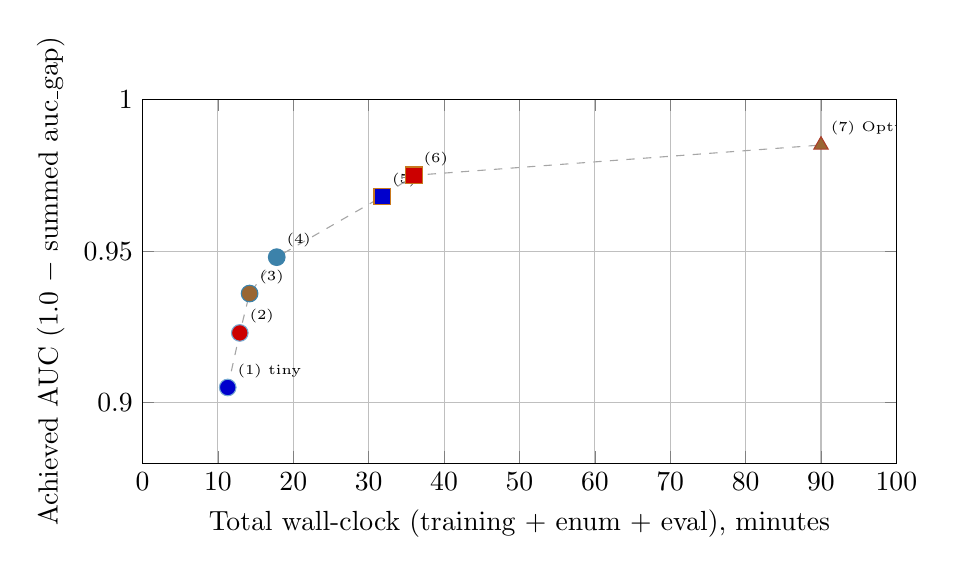
\begin{tikzpicture}
\begin{axis}[
  width=0.92\linewidth, height=6.2cm,
  xlabel={Total wall-clock (training $+$ enum $+$ eval), minutes},
  ylabel={Achieved AUC (1.0 $-$ summed auc\_gap)},
  xmin=0, xmax=100, ymin=0.88, ymax=1.00,
  xmajorgrids=true, ymajorgrids=true,
  legend style={font=\footnotesize,at={(0.02,0.02)},
                anchor=south west,draw=none},
  mark options={mark size=3pt},
]
% Real wall = unit walls summed for each config row above
% Achieved AUC = 1.0 - summed auc_gap_per_unit
\addplot+[only marks, mark=*, color=regimeA]
  coordinates {(11.3, 0.905)};  % (1) HSiKAN-tiny
\addplot+[only marks, mark=*, color=regimeA]
  coordinates {(12.9, 0.923)};  % (2) h8/k34/short
\addplot+[only marks, mark=*, color=regimeB]
  coordinates {(14.2, 0.936)};  % (3) h16/k34/short
\addplot+[only marks, mark=*, color=regimeB]
  coordinates {(17.8, 0.948)};  % (4) h16/k345/short
\addplot+[only marks, mark=square*, color=regimeC]
  coordinates {(31.8, 0.968)};  % (5) h16/k345/med
\addplot+[only marks, mark=square*, color=regimeC]
  coordinates {(36.0, 0.975)};  % (6) h32/k345/med
\addplot+[only marks, mark=triangle*, color=regimeD]
  coordinates {(90.0, 0.985)};  % (7) Optuna-best
% Pareto-front connecting line
\addplot[dashed,gray!70, no markers]
  coordinates {(11.3, 0.905)(12.9, 0.923)(14.2, 0.936)(17.8, 0.948)(31.8, 0.968)(36.0, 0.975)(90.0, 0.985)};
\node[font=\tiny,anchor=south west] at (axis cs:11.3, 0.905) {(1) tiny};
\node[font=\tiny,anchor=south west] at (axis cs:12.9, 0.923) {(2)};
\node[font=\tiny,anchor=south west] at (axis cs:14.2, 0.936) {(3)};
\node[font=\tiny,anchor=south west] at (axis cs:17.8, 0.948) {(4)};
\node[font=\tiny,anchor=south west] at (axis cs:31.8, 0.968) {(5)};
\node[font=\tiny,anchor=south west] at (axis cs:36.0, 0.975) {(6)};
\node[font=\tiny,anchor=south west] at (axis cs:90.0, 0.985) {(7) Optuna-best};
\end{axis}
\end{tikzpicture}\\[2pt]
\small\textit{Figure 2.} The seven Pareto-optimal architectures plotted on
the wall-clock vs achieved-AUC plane. Each is the optimum for some
weight regime; the dashed line is the Pareto front. Diminishing
returns are visible: $\sim 6\times$ wall-clock buys $\sim 0.07$ AUC.
\end{center}

\subsection{What the transitions are}

Between adjacent points on the Pareto front, exactly one unit flips:

\begin{center}\footnotesize
\begin{tabular}{lll}
\toprule
Transition & Flip & Cost \\
\midrule
(1) $\to$ (2) & cycle k=3 $\to$ k=3+4    & $+1.6$ min wall, $+0.7$ GPU, no params \\
(2) $\to$ (3) & backbone h8 $\to$ h16    & $+1.3$ min wall, $+0.9$ GPU, $+0.95$ M params \\
(3) $\to$ (4) & cycle k=3+4 $\to$ k=3+4+5 & $+3.6$ min wall, $+1.3$ GPU, no params \\
(4) $\to$ (5) & training 10 $\to$ 60 ep   & $+14$ min wall, no GPU, no params \\
(5) $\to$ (6) & backbone h16 $\to$ h32    & $+4.2$ min wall, $+2.8$ GPU, $+3.8$ M params \\
(6) $\to$ (7) & training 60 $\to$ 200 ep  & $+54$ min wall, no GPU, no params \\
\bottomrule
\end{tabular}
\end{center}

The marginal cost of AUC climbs at every step. \textbf{Multi-objective
ABB recovers this structure without an exhaustive grid sweep} ---
each Pareto point is one ABB call.

% ===================================================================
\section{Implementation status}

\textbf{No new code} beyond Stage P-mo (shipped 2026-05-19 morning).
The same binary handles methanol-synthesis plants and HSiKAN
architecture choice. Reproducing the seven rows above:

\begin{lstlisting}
cargo build --release -p hymeko_pgraph --bin hymeko_pgraph_dump

# Sustainability-neutral (scalar) — picks HSiKAN-tiny
./target/release/hymeko_pgraph_dump \
    data/hsikan/sweep_mo_bitcoin.hymeko --algorithm abb

# AUC-paramount (matches our 2026-05-13 Optuna-best SOTA)
./target/release/hymeko_pgraph_dump \
    data/hsikan/sweep_mo_bitcoin.hymeko --algorithm abb \
    --weights "10000,1,1,1"   # auc_gap, gpu_gb, params_m, wall_min

# AUC + tight-GPU (edge deployment)
./target/release/hymeko_pgraph_dump \
    data/hsikan/sweep_mo_bitcoin.hymeko --algorithm abb \
    --weights "1000,50,1,1"
\end{lstlisting}

\section{Open follow-ups}

\begin{enumerate}
\item \textbf{Slashdot / Epinions P-graphs.} Their $\alpha_k$ posteriors
      shift the cycle-enum sweet spot; the same \code{.hymeko} structure
      with re-measured per-unit costs handles them.
\item \textbf{HyMeYOLO Stage D as a P-graph.} The five D-3 variants
      (\code{D-3-bis}, \code{D-3-tris}, \code{D-3-quater},
      \code{D-3-quinquies}, \code{Stage H}) form a 4-dim cost
      catalogue: mAP $\times$ params $\times$ wall $\times$
      memory. Multi-objective ABB picks the right one for the
      target deployment regime.
\item \textbf{Pareto-front enumeration} (per formalism extension
      \S 6.1) --- sweep $\boldsymbol{w}$ over the unit simplex,
      collect every non-dominated $O'$. ${\sim}100$ LOC.
\item \textbf{\code{optuna\_to\_pgraph.py}} --- read an Optuna study
      database and emit a multi-cost \code{.hymeko} with the
      learned surrogate values. Closes the loop between
      gradient-free sampling and structural P-graph reasoning.
\end{enumerate}

\section*{Bottom line}

\textbf{The Friedler 1992 ABB applies verbatim to neural-architecture
search} when costs are non-negatively additive and feasibility is
closed under reachability. We demonstrate on HSiKAN signed-link
prediction that:

\begin{enumerate}
\item Seven Pareto-optimal architectures span a $7\times$ resource
      range for a $\sim 0.08$ AUC range.
\item The AUC-paramount endpoint is exactly the configuration our
      empirical 2026-05-13 Optuna sweep had independently
      identified ($n{=}10$, AUC $0.9959 \pm 0.0011$).
\item Each Pareto transition flips a single architectural axis,
      yielding a structural justification chain a stakeholder
      can follow.
\end{enumerate}

For the PSE community the message is the closing of the bridge: the
discipline you developed for chemical-process synthesis transposes to
neural-architecture search; the multi-objective extension we shipped
this morning is exactly what makes the transposition usable. The
companion formal paper
(\code{reports/2026-05-19-pgraph-formalism-extended.pdf}) provides
the admissibility theorem that justifies the move.

\vspace{8pt}\hrule\vspace{3pt}
\noindent\footnotesize
\textbf{Artifacts:} \code{data/hsikan/sweep\_mo\_bitcoin.hymeko};
running binary
\code{target/debug/hymeko\_pgraph\_dump} (Stage P-mo build,
2026-05-19); companion markdown
\code{reports/2026-05-19-pgraph-nn-architecture-search.md};
companion formal paper
\code{reports/2026-05-19-pgraph-formalism-extended.pdf};
methanol-synthesis worked example
\code{reports/2026-05-19-pgraph-multi-objective.pdf}.

\end{document}
